\chapter[Analisi dei risultati]{Analisi quantitativa e qualitativa dei risultati}
\label{chap:risultati}

Le pipeline descritte nel Capitolo~\ref{chap:implementazione} producono mappe che esprimono, per ogni immagine, la deviazione dalla normalità appresa. Il confronto dei risultati permette di esaminare quanto queste risposte siano utili a riconoscere le immagini difettose e a localizzare le anomalie nella categoria \texttt{leather} di MVTec AD. Le metriche descrivono il comportamento sull'intero insieme di test, mentre le mappe e i casi di errore aiutano a comprenderne gli aspetti visivi.

L'analisi collega quindi la discriminazione delle immagini alla qualità della localizzazione, considerando anche i costi osservati nella fase di apprendimento. Il successivo confronto con le pubblicazioni di riferimento colloca gli esiti nel quadro della letteratura, tenendo conto delle differenze tra le configurazioni e i protocolli di valutazione.

\section{Perimetro e criteri di lettura}
\label{sec:cap4-protocollo}

Il confronto utilizza il insieme di addestramento di 245 immagini normali e il insieme di test di 124 immagini descritti nel capitolo precedente. Nel test, 32 immagini sono normali e 92 presentano anomalie. La Tabella~\ref{tab:cap4-difetti} ne riporta la distribuzione nelle cinque tipologie di difetto del materiale, fornendo il riferimento per la lettura degli errori.

\begin{table}[htbp]
\centering
\begin{tabular}{lr}
\hline
Tipo di immagine & Numero \\
\hline
\texttt{good} & 32 \\
\texttt{color} & 19 \\
\texttt{cut} & 19 \\
\texttt{fold} & 17 \\
\texttt{glue} & 19 \\
\texttt{poke} & 18 \\
\hline
Totale & 124 \\
\hline
\end{tabular}
\caption{Composizione del insieme di test della categoria \texttt{leather}.}
\label{tab:cap4-difetti}
\end{table}

I valori riportati provengono dai file di risultato archiviati nel repository e dal relativo rapporto di confronto. I manifesti registrano la configurazione, i dati, i checkpoint, le mappe e il valutatore impiegati. Per questa analisi non sono stati eseguiti nuovi addestramenti: le figure sono state generate dalle mappe archiviate e le matrici di confusione sono state ricostruite dagli stessi punteggi. La verifica di provenienza ha confermato la corrispondenza degli artefatti con gli hash registrati.\footnote{Le esecuzioni originarie sono state effettuate su Linux. La verifica riguarda l'integrità degli artefatti e l'analisi dei risultati archiviati, non una nuova esecuzione dei modelli.}

Come definito nel Capitolo~\ref{chap:introduzione}, l'AUROC a livello di immagine misura la capacità di ordinare le immagini normali e anomale. L'AUROC a livello di pixel valuta l'ordinamento dei pixel, mentre l'AU-PRO valuta la copertura delle regioni annotate al variare dei falsi positivi. Nel protocollo adottato, quest'ultima area è normalizzata nell'intervallo di FPR compreso tra 0 e 0,3. Le due misure di localizzazione sono complementari e non intercambiabili.

Le metriche F1 aggiungono una lettura a soglia. Il massimo F1 è ottenuto selezionando la soglia sul insieme di test: è quindi una misura \emph{oracle}, utile a descrivere il potenziale del punteggio, non una prestazione operativa su dati indipendenti. A livello di pixel il valutatore utilizza un campionamento con passo quattro lungo entrambe le dimensioni e una griglia di 500 soglie; i valori di precisione e richiamo discussi nel seguito si riferiscono a questo stesso campionamento.

Il protocollo comune rende confrontabili gli esiti delle pipeline, ma non annulla le differenze tra esse. PaDiM, RD4AD e FastFlow impiegano feature di una Wide ResNet-50-2 pre-addestrata su ImageNet; CCW-SSIM apprende invece la ricostruzione dalle immagini normali. Risoluzioni, modalità di addestramento e post-elaborazione rimangono quelli documentati nel Capitolo~\ref{chap:implementazione}. Il confronto riguarda dunque sistemi completi nelle configurazioni adottate, non l'effetto isolato della sola funzione di perdita o della sola famiglia metodologica.

\section{Confronto quantitativo complessivo}
\label{sec:cap4-quantitativo}

\subsection{Discriminazione delle immagini e localizzazione}

La Tabella~\ref{tab:cap4-metriche} riassume le metriche principali. Tutti i valori sono espressi nell'intervallo $[0,1]$ e arrotondati a quattro cifre decimali.

\begin{table}[htbp]
\centering
\small
\begin{tabularx}{\textwidth}{Yrrrr}
\hline
Metrica & CCW-SSIM & PaDiM & RD4AD & FastFlow \\
\hline
AUROC immagini & 0,8991 & 1,0000 & 1,0000 & 1,0000 \\
AUROC pixel & 0,9707 & 0,9911 & 0,9942 & 0,9968 \\
AU-PRO & 0,8864 & 0,9786 & 0,9833 & 0,9928 \\
\hline
\end{tabularx}
\caption{Risultati complessivi sul insieme di test \texttt{leather}, con AU-PRO normalizzata fino a FPR pari a 0,3.}
\label{tab:cap4-metriche}
\end{table}

PaDiM, RD4AD e FastFlow raggiungono un'AUROC a livello di immagine pari a 1: i loro punteggi separano completamente le immagini normali da quelle difettose del test. La metrica raggiunge quindi il valore massimo per tutti e tre i metodi e non permette di distinguerli rispetto a questo compito. Il risultato si riferisce ai 124 campioni esaminati e a un'unica esecuzione per pipeline, con seme pseudo-casuale pari a 1024; la generalizzazione a nuove immagini richiede una valutazione ulteriore.

La localizzazione distingue invece le pipeline. FastFlow presenta il valore più alto sia di AUROC pixel sia di AU-PRO, seguito da RD4AD e PaDiM. Rispetto a RD4AD, il vantaggio osservato di FastFlow è di circa 0,26 punti percentuali nell'AUROC pixel e di 0,95 punti percentuali nell'AU-PRO. Tra RD4AD e PaDiM le differenze sono rispettivamente di circa 0,30 e 0,46 punti percentuali. Sono scarti descrittivi: in assenza di ripetizioni e intervalli di incertezza, non ne viene affermata la significatività statistica.

Per CCW-SSIM l'AUROC pixel è pari a 0,9707 e l'AU-PRO a 0,8864. La prima misura indica un buon ordinamento complessivo dei pixel, mentre la seconda evidenzia una copertura delle regioni meno efficace nell'intervallo di falsi positivi considerato. Poiché le due curve integrano grandezze diverse, i valori vanno letti attraverso il loro significato: l'analisi delle mappe permetterà di osservare la copertura dei difetti e le risposte sulla texture normale.

\begin{figure}[htbp]
\centering
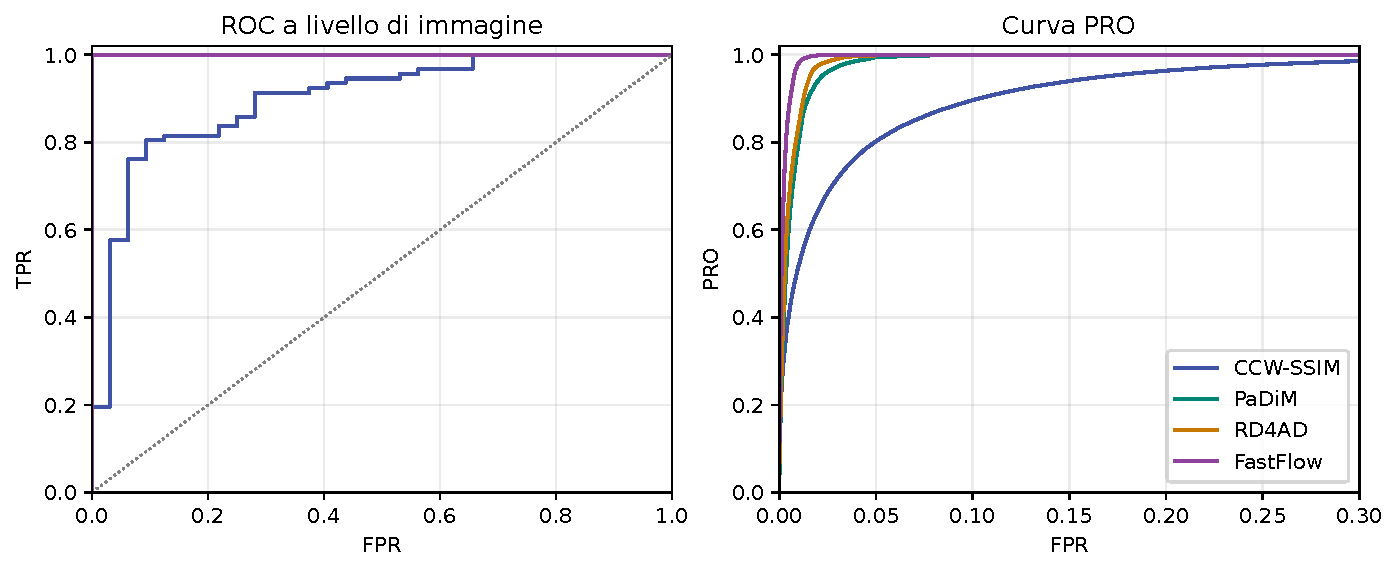
\includegraphics[width=\textwidth]{figure/capitolo_4/curve_roc_pro.pdf}
\caption{Curve ROC a livello di immagine e curve PRO ricavate dai punti archiviati dal valutatore. Le curve ROC di PaDiM, RD4AD e FastFlow si sovrappongono. Le aree riportate nel testo sono quelle salvate nei risultati, non una nuova integrazione dei punti visualizzati.}
\label{fig:cap4-curve}
\end{figure}

\subsection{Risultati a soglia e casi di errore}

Le aree sotto le curve descrivono il comportamento al variare della soglia. Per esaminare le decisioni sulle singole immagini e la segmentazione dei pixel, la Tabella~\ref{tab:cap4-soglie} affianca a queste misure i risultati nei punti operativi selezionati dal valutatore.

\begin{table}[htbp]
\centering
\small
\begin{tabularx}{\textwidth}{Yrrrr}
\hline
Metrica & CCW-SSIM & PaDiM & RD4AD & FastFlow \\
\hline
F1 massimo immagini & 0,9081 & 1,0000 & 1,0000 & 1,0000 \\
F1 massimo pixel & 0,3840 & 0,4243 & 0,4981 & 0,6161 \\
FPR con TPR $\geq 95\%$ & 0,5312 & 0,0000 & 0,0000 & 0,0000 \\
\hline
\end{tabularx}
\caption{Metriche a soglia. Le soglie di massimo F1 sono selezionate sul insieme di test; l'FPR dell'ultima riga riguarda la classificazione delle immagini.}
\label{tab:cap4-soglie}
\end{table}

Alla soglia che massimizza l'F1 a livello di immagine, CCW-SSIM identifica 84 immagini difettose e ne omette 8; classifica correttamente 23 immagini normali e segnala come anomale le altre 9. La precisione è circa 0,9032 e il richiamo circa 0,9130. Per gli altri tre metodi, alla rispettiva soglia ottimale, non si osservano falsi positivi o falsi negativi a livello di immagine.

Il comportamento cambia imponendo un richiamo di almeno il 95\%: per CCW-SSIM l'FPR sale a 0,5312, corrispondente a 17 immagini normali segnalate su 32. Il valore illustra il costo, su questo insieme di dati, della riduzione delle omissioni. Non va confuso con i nove falsi positivi alla soglia di massimo F1, poiché i due criteri selezionano punti operativi differenti.

A livello di pixel, i massimi F1 sono sensibilmente inferiori alle AUROC pixel. Un buon ordinamento dei punteggi non implica infatti che esista una soglia capace di delineare il difetto con precisione elevata: possono rimanere aloni, risposte sullo sfondo o parti della regione non rilevate. La Tabella~\ref{tab:cap4-precisione} esplicita questo compromesso.

\begin{table}[htbp]
\centering
\begin{tabular}{lrrr}
\hline
Modello & Precisione pixel & Richiamo pixel & F1 pixel \\
\hline
CCW-SSIM & 0,3704 & 0,3986 & 0,3840 \\
PaDiM & 0,3159 & 0,6463 & 0,4243 \\
RD4AD & 0,3999 & 0,6603 & 0,4981 \\
FastFlow & 0,5233 & 0,7488 & 0,6161 \\
\hline
\end{tabular}
\caption{Precisione e richiamo alla soglia globale di massimo F1 pixel di ciascun modello, sul campionamento previsto dal valutatore.}
\label{tab:cap4-precisione}
\end{table}

PaDiM recupera una quota di pixel anomali maggiore di CCW-SSIM, ma presenta una precisione inferiore. RD4AD migliora entrambi i valori rispetto a PaDiM, mentre FastFlow ottiene il miglior compromesso osservato. Anche per FastFlow una precisione di 0,5233 indica che, alla soglia considerata, una parte consistente dei pixel segnalati non appartiene alle annotazioni del difetto. L'esito favorevole nel riconoscimento dell'immagine non deve quindi essere trasferito automaticamente alla precisione della segmentazione.

L'interpretazione di questi punti operativi dipende dalla scala del punteggio di ciascun modello. Il valutatore normalizza punteggi originariamente differenti, che non rappresentano probabilità calibrate: le soglie numeriche vanno quindi riferite alla rispettiva pipeline. Il loro uso su dati futuri richiederebbe una selezione su un insieme di validazione indipendente, come discusso nella Sezione~\ref{sec:cap4-limiti}.

\subsection{Costi osservati nella fase di apprendimento}

Accanto alle prestazioni, i tempi registrati descrivono il lavoro necessario ad adattare ciascuna pipeline al materiale. La Tabella~\ref{tab:cap4-costi} li mette in relazione con i passaggi sui dati e gli aggiornamenti dei parametri, distinguendo la stima statistica di PaDiM dall'ottimizzazione iterativa degli altri modelli.

\begin{table}[htbp]
\centering
\small
\begin{tabularx}{\textwidth}{Yrrr}
\hline
Pipeline & Passaggi sui dati & Aggiornamenti & Tempo (min) \\
\hline
CCW-SSIM & 200 & 49\,000 & 374,1 \\
PaDiM & 1 & 0 & 0,2 \\
RD4AD & 200 & 3\,200 & 8,7 \\
FastFlow & 200 & 6\,200 & 11,5 \\
\hline
\end{tabularx}
\caption{Tempi della fase di apprendimento o adattamento registrati nelle esecuzioni su GPU NVIDIA RTX 4070 Ti. Per PaDiM l'adattamento consiste nella stima statistica, senza aggiornamenti tramite discesa del gradiente.}
\label{tab:cap4-costi}
\end{table}

PaDiM richiede il tempo di adattamento più basso, mentre CCW-SSIM presenta quello più alto. RD4AD e FastFlow si collocano tra questi estremi. I tempi non rappresentano un confronto a parità di lavoro: differiscono il numero di aggiornamenti, il batch, la precisione numerica, la gestione delle patch e l'architettura. Inoltre, i metodi basati su feature utilizzano un pre-addestramento esterno, il cui costo non è incluso nelle misure.

Il risultato consente quindi di discutere il costo locale di preparazione delle pipeline, non la loro efficienza complessiva. Non sono disponibili qui misure omogenee di latenza, numero di immagini elaborate per unità di tempo e memoria durante l'inferenza; il tempo di addestramento non può sostituirle né verificare le dichiarazioni di velocità dei lavori originali.

\section{Analisi qualitativa e confronto caso per caso}
\label{sec:cap4-qualitativo}

Le differenze tra AUROC, AU-PRO e F1 rendono utile osservare come i punteggi si distribuiscano nelle immagini. Le figure affiancano l'immagine originale, la maschera annotata e le quattro mappe di anomalia. Il contorno verde sulle mappe indica il riferimento annotato, non una segmentazione prodotta dal modello. Per mantenere una scala coerente tra esempi dello stesso metodo, la visualizzazione applica una normalizzazione min--max basata sull'intero insieme delle mappe di test di ciascuna pipeline:
\begin{equation}
\widetilde{S}_m(x)=\frac{S_m(x)-a_m}{b_m-a_m},
\end{equation}
dove $a_m$ e $b_m$ sono rispettivamente il minimo e il massimo delle mappe del modello $m$. Non viene normalizzata ogni immagine separatamente. Questa trasformazione serve soltanto alla visualizzazione e non modifica le metriche archiviate. Non coincide necessariamente con gli estremi ricavati dal campionamento usato per l'F1 pixel.

Poiché ciascun modello mantiene una propria scala, la stessa tonalità in due pannelli non esprime una probabilità di anomalia equivalente. Il confronto visivo riguarda posizione, forma ed estensione delle risposte. La classificazione dipende invece dal massimo della mappa e dalla soglia globale del modello: una risposta su parte del difetto può essere sufficiente a segnalare l'immagine, mentre una zona luminosa in un campione normale va interpretata rispetto a quella soglia. I conteggi per tipologia riportati nel seguito descrivono le decisioni sulle immagini; la qualità della segmentazione è valutata dalle metriche a livello di pixel e regionali.

Per ciascuna tipologia di difetto è stato scelto il primo file in ordine lessicografico, \texttt{000.png}. La regola rende la selezione riproducibile, ma non garantisce che i campioni siano rappresentativi dell'intera tipologia. Sono aggiunti due esempi diagnostici: l'immagine normale con il massimo punteggio CCW-SSIM e un difetto omesso da tale modello. La Tabella~\ref{tab:cap4-fn} fornisce il contesto quantitativo delle omissioni sull'intero insieme di test, prima della lettura dei singoli esempi.

\begin{table}[htbp]
\centering
\begin{tabular}{lrrrr}
\hline
Difetto & CCW-SSIM & PaDiM & RD4AD & FastFlow \\
\hline
\texttt{color} & 2/19 & 0/19 & 0/19 & 0/19 \\
\texttt{cut} & 1/19 & 0/19 & 0/19 & 0/19 \\
\texttt{fold} & 0/17 & 0/17 & 0/17 & 0/17 \\
\texttt{glue} & 4/19 & 0/19 & 0/19 & 0/19 \\
\texttt{poke} & 1/18 & 0/18 & 0/18 & 0/18 \\
\hline
Totale & 8/92 & 0/92 & 0/92 & 0/92 \\
\hline
\end{tabular}
\caption{Falsi negativi a livello di immagine sul numero di campioni difettosi. Per ogni modello si mantiene la stessa soglia globale di massimo F1 immagini, senza ottimizzarla per tipologia.}
\label{tab:cap4-fn}
\end{table}

\subsection{Alterazione cromatica: \texttt{color}}

Nel campione \texttt{color/000.png} il difetto occupa una piccola zona nella parte inferiore destra dell'immagine. PaDiM, RD4AD e FastFlow producono una risposta riconoscibile nella posizione annotata. PaDiM presenta una distribuzione più regolare e a blocchi, RD4AD una risposta più compatta, mentre FastFlow evidenzia il difetto con un nucleo intenso e una risposta anche nelle aree circostanti. La mappa CCW-SSIM è maggiormente influenzata dalla tessitura diffusa del materiale e mostra un contrasto locale meno evidente.

Il contrasto locale poco evidente di CCW-SSIM si accompagna al riconoscimento di 17 delle 19 immagini \texttt{color} alla soglia globale di massimo F1. L'esempio invita quindi a esaminare la relazione tra risposta cromatica e tessitura del materiale. Il contributo specifico del colore alla funzione di perdita sarà discusso nel confronto con la fonte, poiché la sua misura richiede un'ablazione controllata rispetto alla variante priva di tale componente.

\begin{figure}[htbp]
\centering
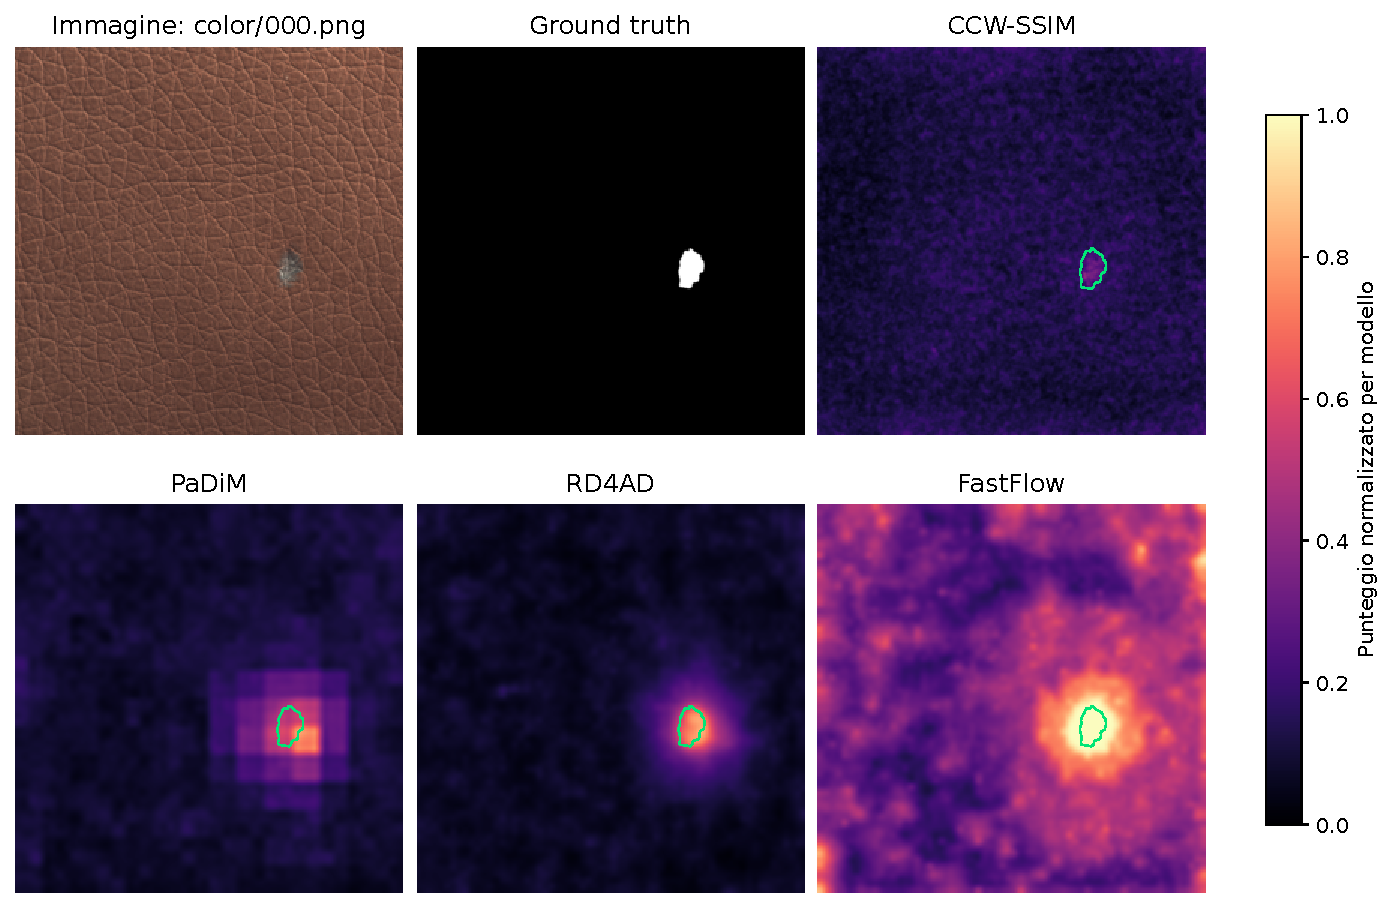
\includegraphics[width=\textwidth]{figure/capitolo_4/leather_color_000.pdf}
\caption{Confronto qualitativo sul campione \texttt{color/000.png}. Il contorno verde rappresenta la regione annotata.}
\label{fig:cap4-color}
\end{figure}

\subsection{Taglio: \texttt{cut}}

Il campione \texttt{cut/000.png} contiene un difetto sottile, prevalentemente orizzontale. I tre metodi basati su feature rispondono nell'area corretta, ma la regione ad alto punteggio si estende oltre la geometria del taglio. Questo esempio rende visibile la distinzione tra individuare la posizione del difetto e ricostruirne precisamente il contorno. La risposta PaDiM è più squadrata; quelle di RD4AD e FastFlow sono più continue, pur mantenendo un'estensione superiore alla maschera.

CCW-SSIM presenta una mappa granulare nella quale il difetto emerge meno nettamente rispetto allo sfondo; sull'intera tipologia viene omessa una sola immagine su 19. Il caso richiama soprattutto l'attenzione sui bordi: per una struttura sottile, ricampionamento e filtraggio possono influenzare l'estensione visibile della risposta. Gli esperimenti disponibili descrivono l'esito della pipeline completa e non isolano il contributo di questi passaggi.

\begin{figure}[htbp]
\centering
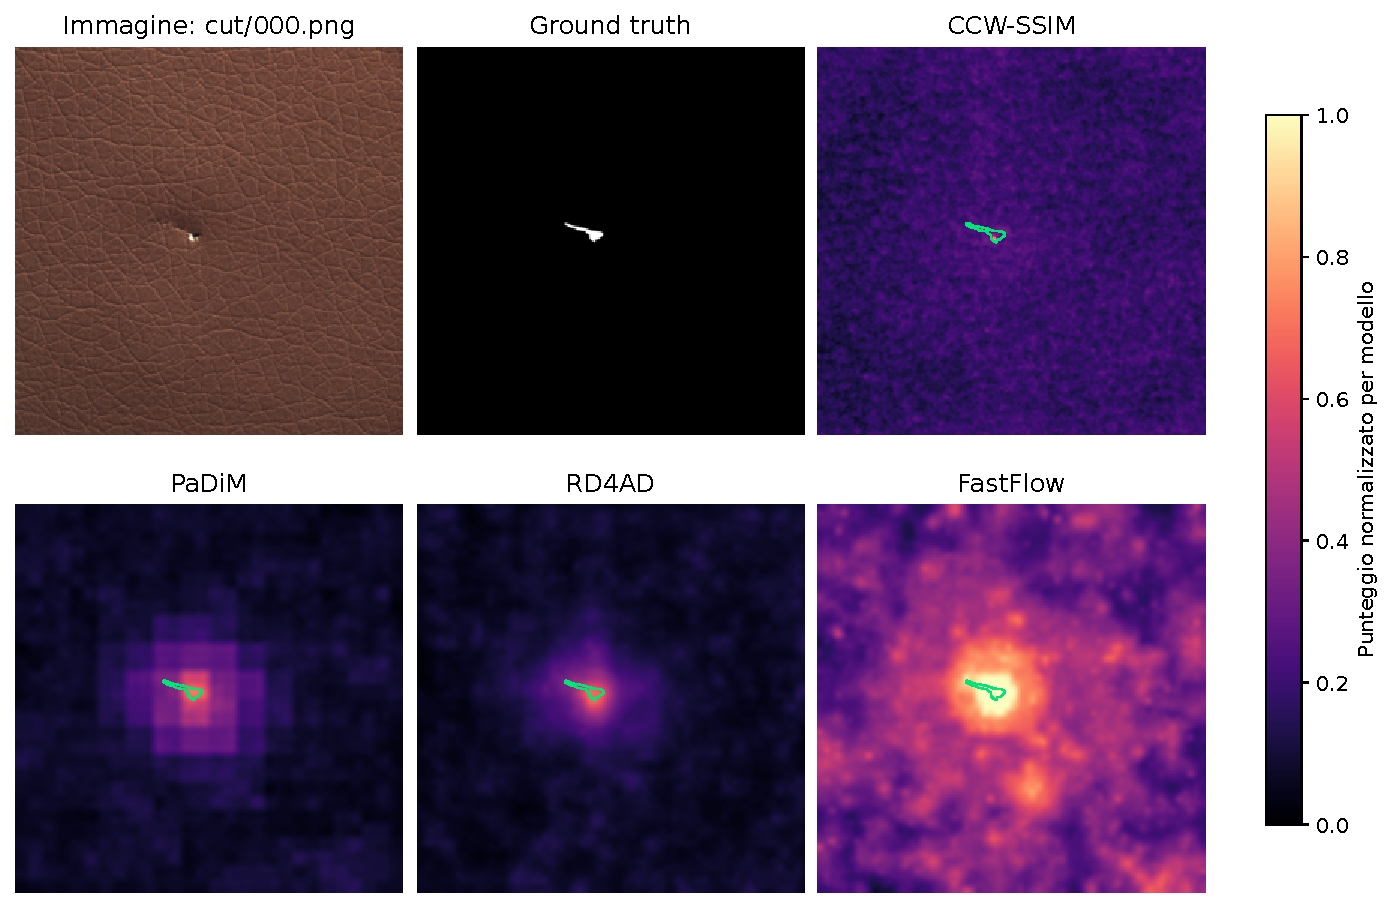
\includegraphics[width=\textwidth]{figure/capitolo_4/leather_cut_000.pdf}
\caption{Confronto sul campione \texttt{cut/000.png}: la risposta nell'area corretta non implica una segmentazione aderente al taglio.}
\label{fig:cap4-cut}
\end{figure}

\subsection{Piega: \texttt{fold}}

In \texttt{fold/000.png} la regione difettosa è allungata e si trova nella parte superiore sinistra. PaDiM, RD4AD e FastFlow individuano tale zona, con risposte che ne comprendono anche il contesto. CCW-SSIM conserva una risposta diffusa alla texture e un'evidenza locale meno netta alla scala di visualizzazione adottata.

CCW-SSIM riconosce tutte le 17 immagini \texttt{fold} alla soglia di massimo F1 immagini. La risposta diffusa osservata nel pannello convive quindi con un riconoscimento completo della tipologia nel test. Il caso mostra come il massimo della mappa possa sostenere la decisione sull'immagine anche quando la regione difettosa emerge con un contrasto visivo limitato.

\begin{figure}[htbp]
\centering
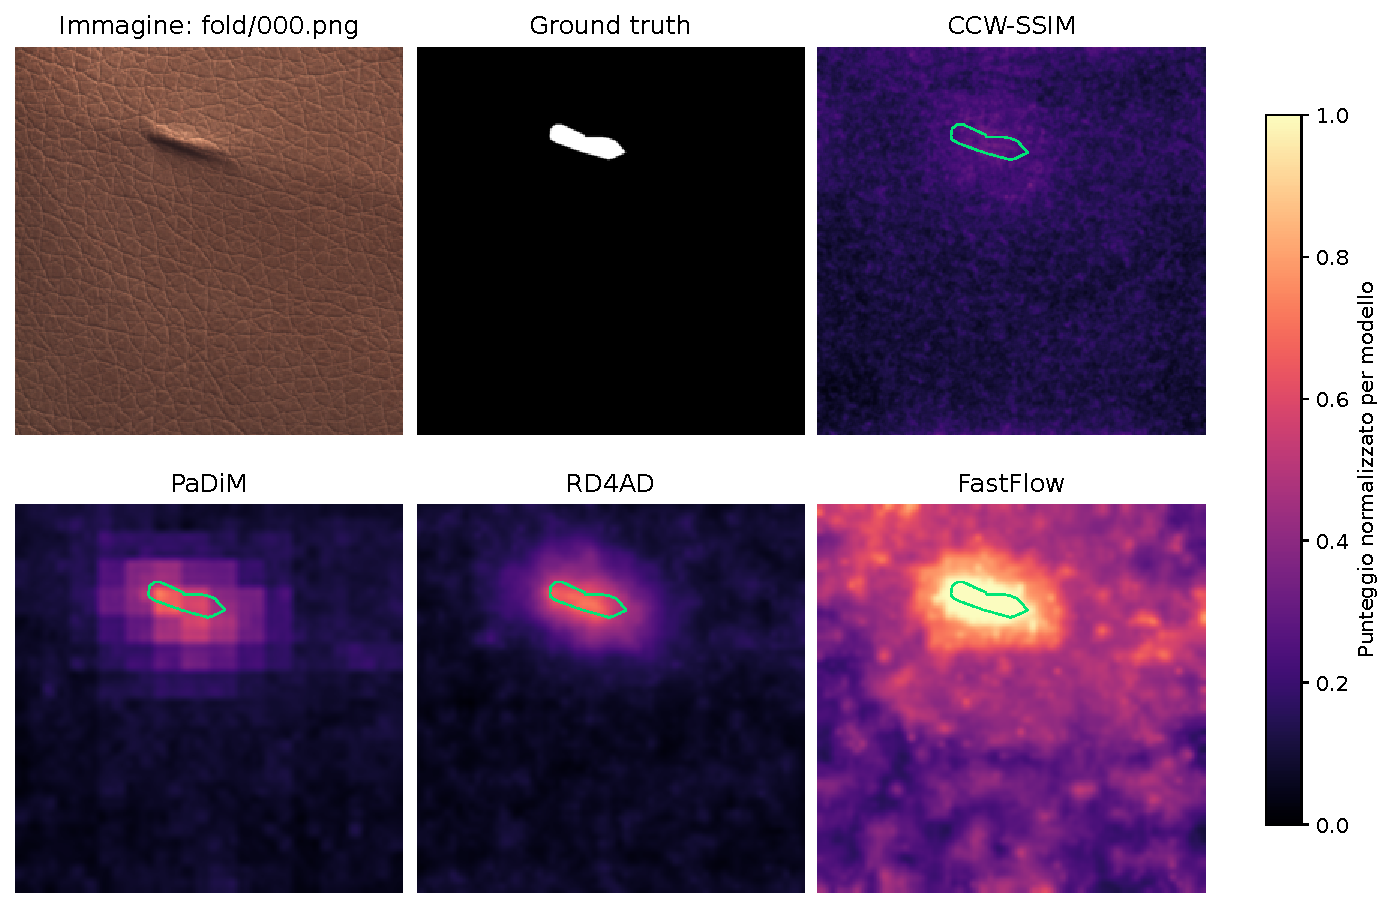
\includegraphics[width=\textwidth]{figure/capitolo_4/leather_fold_000.pdf}
\caption{Confronto sul campione \texttt{fold/000.png}, caratterizzato da un difetto allungato.}
\label{fig:cap4-fold}
\end{figure}

\subsection{Residuo di colla: \texttt{glue}}

Nel campione \texttt{glue/000.png} la regione annotata è compatta e presenta variazioni di aspetto al suo interno. Le mappe PaDiM e RD4AD rispondono in modo non uniforme nella zona difettosa; FastFlow produce un nucleo più estesamente intenso. CCW-SSIM mostra risposte soprattutto su piccole porzioni e variazioni locali, senza riprodurre con altrettanta evidenza l'intera area annotata.

Quattro degli otto falsi negativi di CCW-SSIM appartengono a \texttt{glue}: sono quattro omissioni su 19 campioni, il numero più alto tra le tipologie considerate. La Figura~\ref{fig:cap4-glue-fn} aggiunge \texttt{glue/001.png}, il primo falso negativo in ordine lessicografico di questa tipologia. Il campione è selezionato per documentare un errore effettivo, non per rappresentare un caso medio. La sua omissione è determinata dal punteggio globale dell'immagine alla soglia considerata, non dall'assenza di qualunque risposta visibile sulla mappa.

\begin{figure}[htbp]
\centering
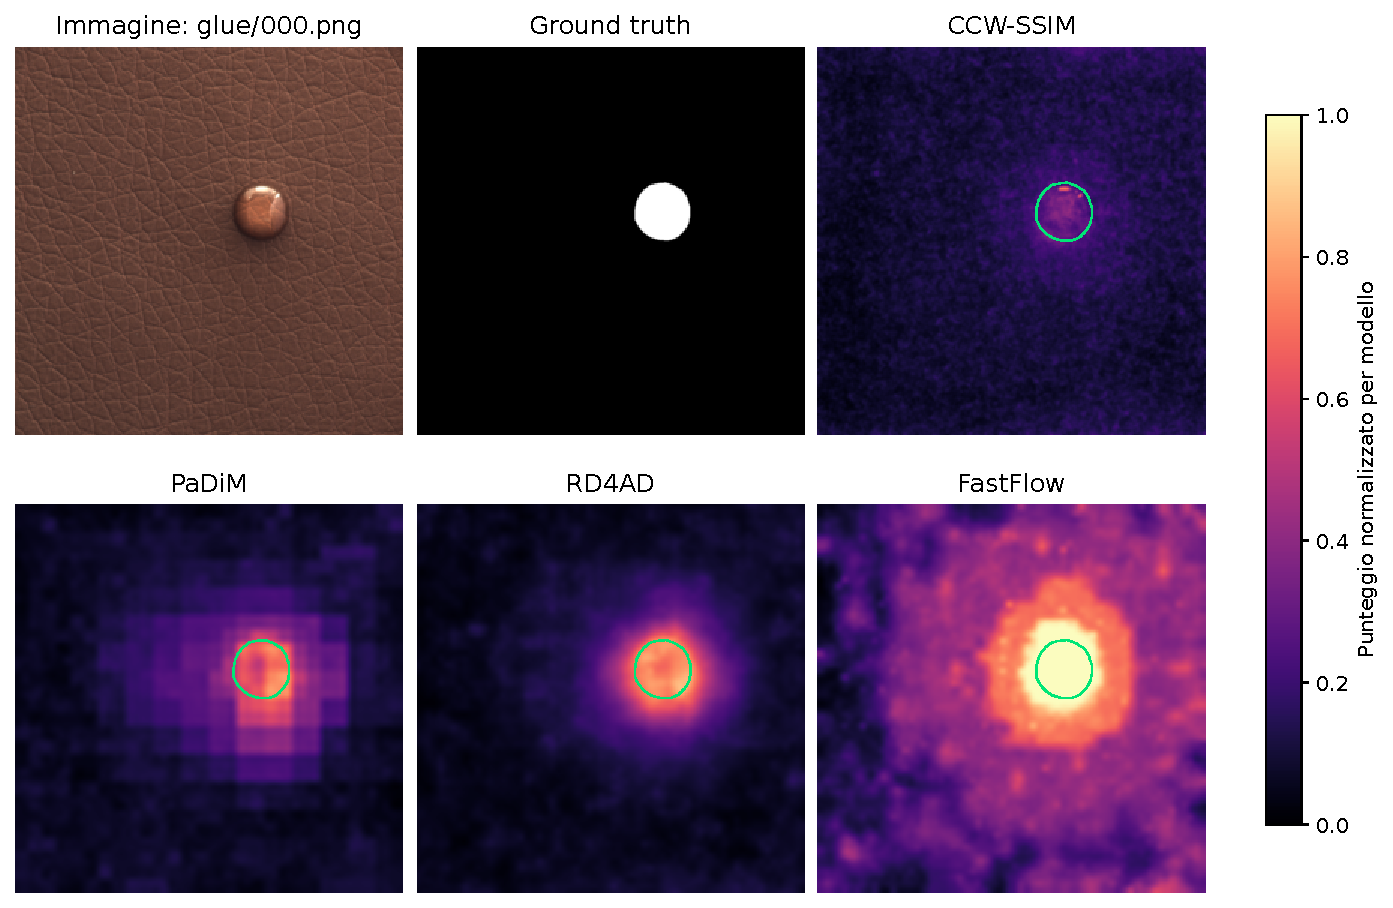
\includegraphics[width=\textwidth]{figure/capitolo_4/leather_glue_000.pdf}
\caption{Confronto sul campione \texttt{glue/000.png}.}
\label{fig:cap4-glue}
\end{figure}

\begin{figure}[htbp]
\centering
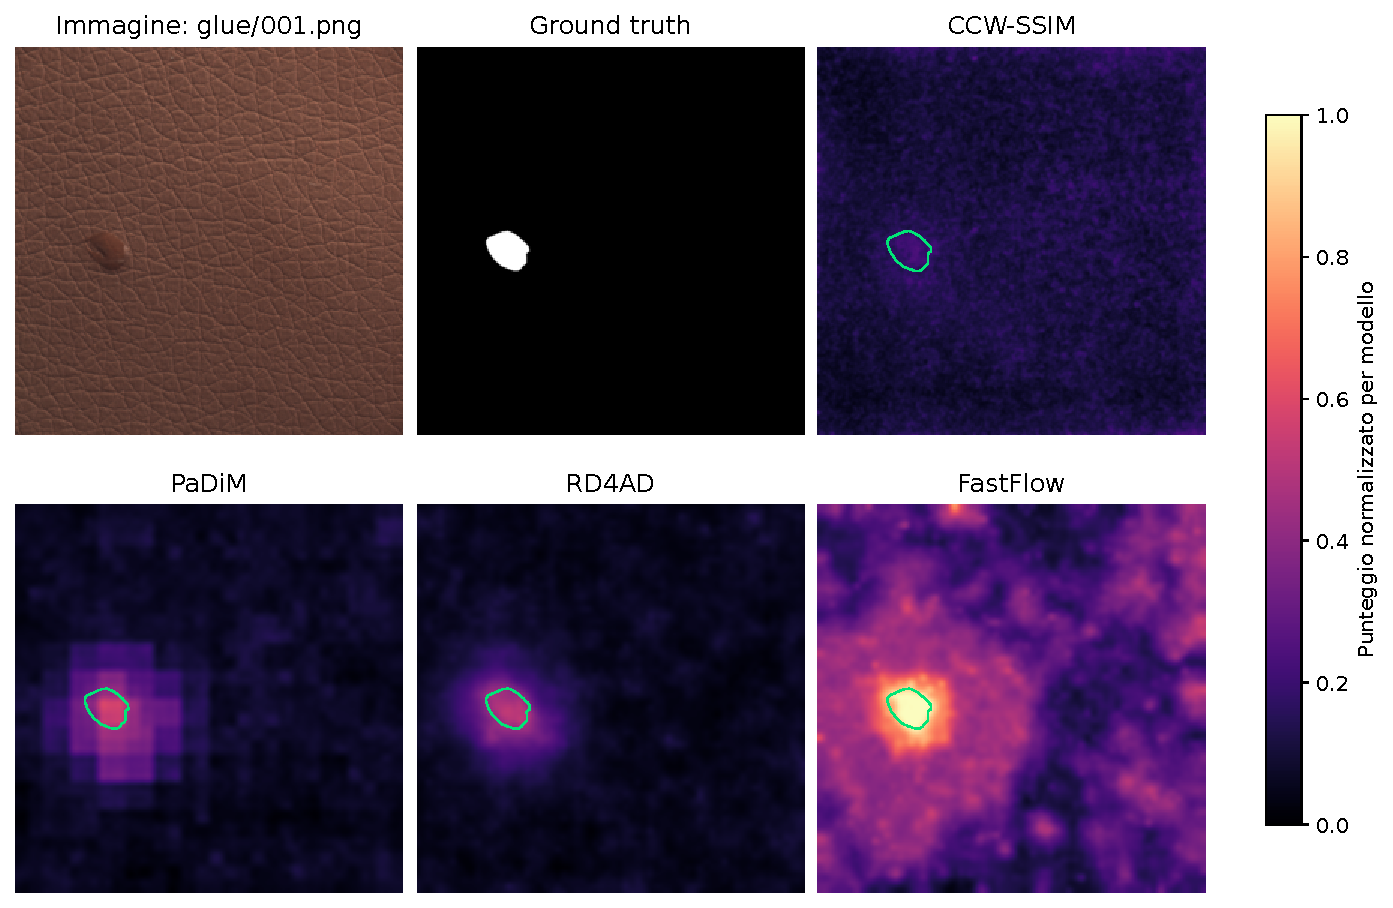
\includegraphics[width=\textwidth]{figure/capitolo_4/leather_glue_001.pdf}
\caption{Campione \texttt{glue/001.png}, falso negativo di CCW-SSIM alla soglia globale di massimo F1 immagini. Gli altri tre modelli lo classificano correttamente alle rispettive soglie.}
\label{fig:cap4-glue-fn}
\end{figure}

\subsection{Perforazione: \texttt{poke}}

In \texttt{poke/000.png} il difetto è piccolo e si trova nella parte inferiore sinistra. I tre modelli basati su feature presentano una risposta localizzata, più ampia del riferimento annotato. CCW-SSIM mostra una risposta meno distinguibile dalla texture circostante. Per un difetto di dimensioni ridotte, un'estensione della mappa oltre il contorno può incidere sulla precisione anche quando il centro della risposta è corretto.

CCW-SSIM omette una delle 18 immagini \texttt{poke} alla soglia globale scelta, mentre gli altri metodi le riconoscono tutte. Rispetto agli esempi precedenti, la piccola area annotata mette in evidenza il peso delle risposte circostanti: una localizzazione centrata sul difetto può comunque includere una quota rilevante di pixel normali.

\begin{figure}[htbp]
\centering
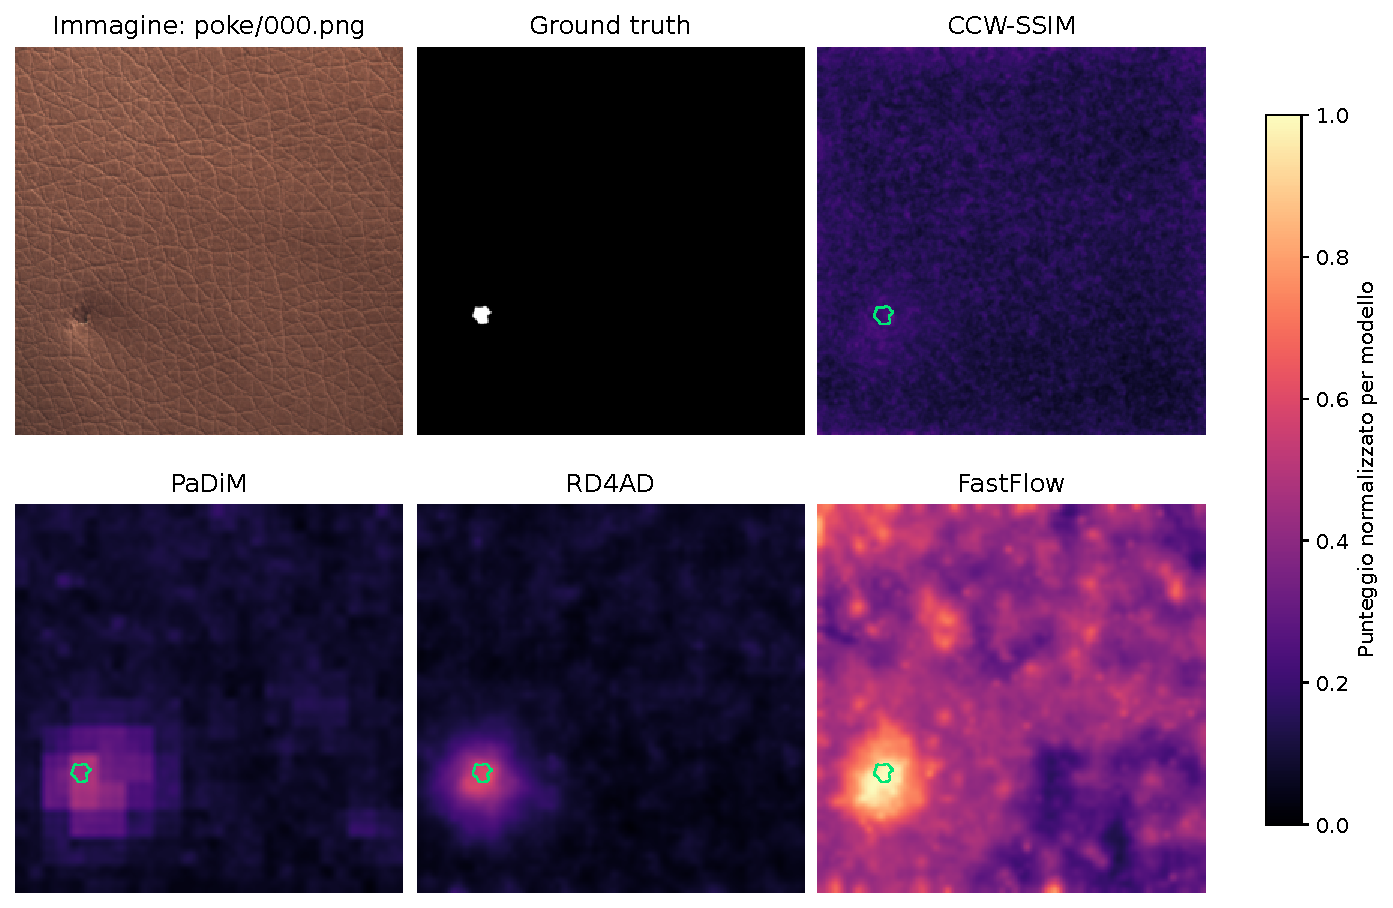
\includegraphics[width=\textwidth]{figure/capitolo_4/leather_poke_000.pdf}
\caption{Confronto sul campione \texttt{poke/000.png}, con difetto di piccole dimensioni.}
\label{fig:cap4-poke}
\end{figure}

\subsection{Immagine normale e falso positivo}

Il campione \texttt{good/030.png} è l'immagine normale con il massimo punteggio CCW-SSIM. La maschera di riferimento è vuota. La mappa CCW-SSIM contiene risposte diffuse alla tessitura e picchi locali: il massimo supera la soglia di classificazione e rende questa immagine uno dei nove falsi positivi del modello.

Anche le altre pipeline producono mappe non uniformi su questa immagine normale, ma i rispettivi punteggi rimangono al di sotto delle soglie globali di massimo F1 immagini. Per CCW-SSIM, invece, il picco determina una segnalazione errata. Il caso collega così la risposta alla tessitura alla scelta di aggregare la mappa mediante massimo e motiva un possibile approfondimento su aggregazioni alternative, il cui beneficio rimane da verificare.

\begin{figure}[htbp]
\centering
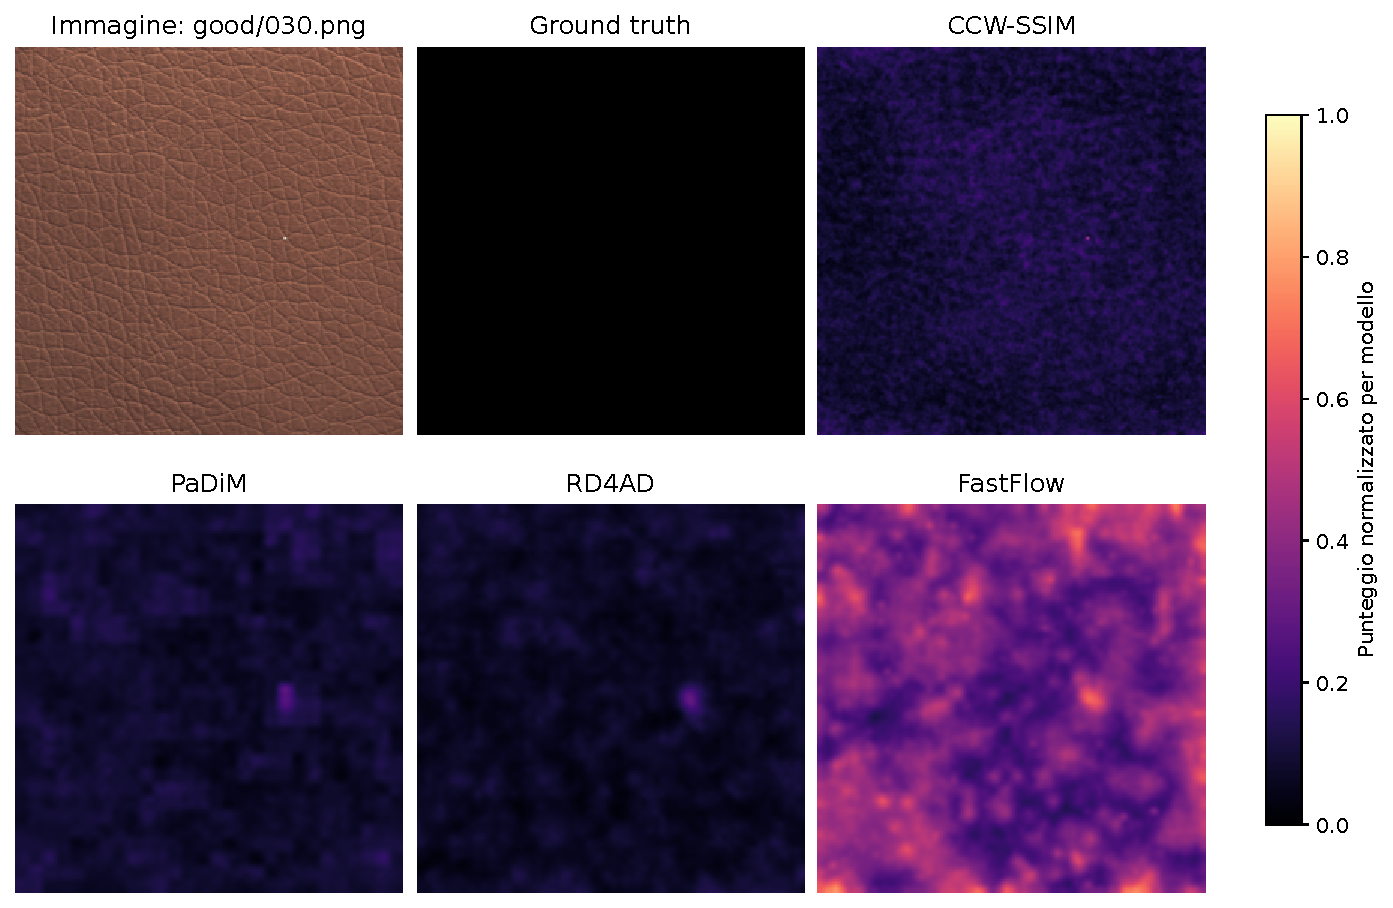
\includegraphics[width=\textwidth]{figure/capitolo_4/leather_good_030.pdf}
\caption{Immagine normale \texttt{good/030.png}, falso positivo di CCW-SSIM alla soglia di massimo F1 immagini. L'assenza di regioni annotate è mostrata dalla maschera vuota.}
\label{fig:cap4-good}
\end{figure}

\subsection{Sintesi della lettura qualitativa}

Negli esempi selezionati, PaDiM mostra risposte più regolari e a blocchi, RD4AD risposte più compatte e FastFlow nuclei intensi accompagnati, in alcuni casi, da un'attivazione più diffusa del contesto. CCW-SSIM presenta mappe più granulari, nelle quali la texture normale rimane visibile e il contrasto del difetto può essere ridotto. Queste descrizioni riguardano i pannelli esaminati e non sostituiscono un'analisi quantitativa di tutte le mappe.

La lettura delle figure è coerente con due risultati complessivi: i metodi basati su feature individuano la zona difettosa nei campioni mostrati, ma mantengono imprecisioni di estensione; CCW-SSIM può segnalare un difetto senza coprirlo interamente e può attribuire un punteggio elevato anche a un'immagine normale. Non è invece giustificato attribuire le differenze alla sola risoluzione, al solo pre-addestramento o alla sola funzione di perdita: tali fattori non sono stati variati separatamente.

\FloatBarrier

\section{Confronto con le pubblicazioni di riferimento}
\label{sec:cap4-letteratura}

Le metriche e gli esempi visivi delineano il comportamento delle pipeline nel caso di studio. Per metterlo in relazione con le proposte originali, occorre confrontare sia i valori pubblicati sia le condizioni in cui sono stati ottenuti. Si considerano quindi i risultati di \texttt{leather}, quando disponibili, mantenendoli distinti dalle medie sulle quindici categorie di MVTec AD.

La Tabella~\ref{tab:cap4-paper} affianca i risultati locali ai valori pubblicati per le metriche con una corrispondenza nominale. Gli scarti sono espressi in punti percentuali e sono soltanto descrittivi: la tabella non presuppone identità dei protocolli. CCW-SSIM viene discusso separatamente, poiché la diversa definizione dell'area impedisce di riportare uno scarto equivalente.

\begin{table}[htbp]
\centering
\small
\begin{tabularx}{\textwidth}{lYrrr}
\hline
Metodo & Metrica & Fonte (\%) & Locale (\%) & Scarto (p.p.) \\
\hline
PaDiM & AUROC pixel & 99,20 & 99,11 & $-0,09$ \\
 & PRO & 97,80 & 97,86 & $+0,06$ \\
RD4AD & AUROC immagini & 100,00 & 100,00 & $0,00$ \\
 & AUROC pixel & 99,40 & 99,42 & $+0,02$ \\
 & PRO & 99,10 & 98,33 & $-0,77$ \\
FastFlow & AUROC immagini & 100,00 & 100,00 & $0,00$ \\
 & AUROC pixel & 99,50 & 99,68 & $+0,18$ \\
\hline
\end{tabularx}
\caption{Riscontro descrittivo su \texttt{leather} con le tabelle originali di PaDiM, Reverse Distillation e FastFlow. La misura regionale locale è l'AU-PRO definita nel protocollo dell'elaborato; la corrispondenza esatta dei valutatori non è accertata per tutte le fonti. Lo scarto è locale meno fonte e non indica significatività statistica.}
\label{tab:cap4-paper}
\end{table}

\subsection{PaDiM}

Nella Tabella III del lavoro di Defard et al.~\cite{Defard_et_al._2021}, la configurazione PaDiM con Wide ResNet-50-2 e 550 dimensioni riporta per \texttt{leather} un'AUROC pixel del 99,2\% e un PRO-score del 97,8\%. I valori locali, rispettivamente 99,11\% e 97,86\%, sono prossimi a quelli pubblicati. Questo riscontro sostiene la coerenza del comportamento di localizzazione osservato.

Per interpretare questo allineamento occorre considerare il preprocessing. Il lavoro originale prevede ridimensionamento a 256 pixel e ritaglio centrale a 224, mentre la configurazione locale ridimensiona direttamente a 224. Possono inoltre differire dettagli del valutatore e della selezione delle feature.

La differenza di preprocessing è concreta: il ritaglio conserva la scala della parte centrale dell'immagine ridimensionata e ne esclude i margini, mentre il ridimensionamento diretto mantiene l'intero campo visivo a una scala diversa. Questo modifica la corrispondenza tra texture, difetti e posizioni delle feature statistiche. È un fattore plausibile per leggere i piccoli scarti, ma il suo effetto non è stato misurato separatamente. Anche il rapido adattamento locale è coerente con l'assenza di addestramento della rete descritta dalla pubblicazione; non costituisce invece una verifica dei suoi tempi assoluti, ottenuti con hardware e implementazione differenti.

\subsection{Reverse Distillation}

Le Tabelle 1 e 2 di Deng e Li~\cite{Deng_et_al._2022} riportano per \texttt{leather}, alla risoluzione di 256 pixel, un'AUROC immagini del 100\%, un'AUROC pixel del 99,4\% e un PRO del 99,1\%. Nell'esecuzione locale RD4AD raggiunge rispettivamente il 100\%, il 99,42\% e il 98,33\%.

La discriminazione delle immagini e l'AUROC pixel risultano quindi prossime ai valori pubblicati, mentre tra i due valori regionali vi è uno scarto descrittivo di circa 0,77 punti percentuali. La verifica del codice ufficiale \cite{Deng_RD4AD_code_2022} accerta però protocolli differenti: il riferimento calcola il PRO per ciascuna immagine difettosa, con 200 soglie, poi media le aree; il valutatore locale costruisce un'unica curva globale sulle 124 immagini, includendo quelle normali. Le due procedure pesano diversamente regioni e falsi positivi. Lo scarto non misura quindi una perdita del modello a parità di valutazione.

I principali parametri di addestramento coincidono con quelli dichiarati nella fonte: 200 epoche, batch da 16 immagini e Adam con tasso di apprendimento pari a 0,005 e coefficienti $(0{,}5,0{,}999)$. Il codice ufficiale valuta e filtra a $256\times256$, mentre qui le mappe sono interpolate a $1024\times1024$ prima del filtro con $\sigma=4$: lo stesso valore numerico non corrisponde alla stessa scala spaziale. È verificata la differenza di procedura, non il suo contributo quantitativo al risultato. Per isolare le cause servirebbe applicare entrambi i protocolli a predizioni omogenee, senza modificare retrospettivamente il confronto locale.

\subsection{FastFlow}

La Tabella 2 di Yu et al.~\cite{Yu_et_al._2021} riporta per \texttt{leather} un'AUROC immagini del 100\% e un'AUROC pixel del 99,5\%. L'esecuzione locale ottiene il 100\% e il 99,68\%. I risultati confermano, nel perimetro considerato, la buona separazione delle immagini e l'elevata capacità di localizzazione descritta nella pubblicazione.

Il porting adottato utilizza la configurazione Wide ResNet-50-2 documentata nel Capitolo~\ref{chap:implementazione}, mentre la pubblicazione considera diverse architetture di estrazione delle feature. L'identità completa con la configurazione sottostante al valore pubblicato non è stabilita. Il lieve scarto positivo va quindi interpretato insieme alle scelte di implementazione e di apprendimento.

La fonte descrive 500 epoche e batch da 32, mentre il progetto usa 200 epoche e batch da 8, mantenendo tasso di apprendimento $10^{-3}$ e decadimento dei pesi $10^{-5}$. Cambiano così il regime di ottimizzazione e il numero di aggiornamenti. Il vantaggio descrittivo di 0,18 punti percentuali non può essere attribuito a una modifica specifica senza prove controllate. Il confronto sostiene la capacità di produrre punteggi discriminanti nel caso di studio; le proprietà di efficienza in inferenza discusse dalla pubblicazione richiederebbero invece misure di latenza e numero di immagini elaborate per unità di tempo, distinte dai tempi di addestramento qui riportati.

\subsection{CCW-SSIM e il ruolo dell'informazione cromatica}

La fonte di Berasi~\cite{Berasi_2023} ha come obiettivo centrale l'integrazione dell'informazione cromatica nella misura strutturale utilizzata da un autoencoder. Il confronto tra varianti della funzione di perdita è quindi essenziale per valutarne il contributo. Il presente lavoro include CCW-SSIM nel confronto con tre pipeline basate su feature, ma non contiene l'ablazione controllata rispetto alla variante CW-SSIM. Non può pertanto confermare né confutare direttamente il vantaggio della componente cromatica.

Un'ulteriore distinzione riguarda le metriche. La Tabella 1 della fonte riporta per \texttt{leather} il valore 0,982 relativo alla curva ROC; nella sezione sulle prestazioni, la fonte specifica una normalizzazione dell'area limitata a FPR pari a 0,3. La nostra AUROC pixel, pari a 0,9707, integra invece la curva completa. Anche l'AU-PRO locale non è la stessa misura, perché integra la copertura delle regioni anziché il tasso di veri positivi pixel. Nessuno dei due valori consente quindi un confronto diretto con 0,982.

Il risultato locale di CCW-SSIM va dunque letto rispetto alla pipeline utilizzata. La fonte distingue il beneficio cromatico all'interno dell'approccio ricostruttivo dal confronto con metodi più sofisticati dello stato dell'arte. Per approfondire tale beneficio nel progetto occorre mantenere fissi architettura, dati e valutatore e variare la componente della perdita.

La verifica del percorso effettivo individua inoltre differenze nella componente cromatica, esplicitate nel Capitolo~\ref{chap:implementazione}: errore quadratico anziché distanza euclidea, aggregazione globale durante l'addestramento e coefficienti differenti in inferenza. Queste scelte preservano l'idea di combinare struttura e colore, ma non permettono di trasferire automaticamente alla variante locale il beneficio cromatico dimostrato dalla fonte.

Per approfondire le scelte di implementazione, un test diagnostico del checkpoint esistente, senza addestramento e senza sostituire le mappe ufficiali, ha elaborato dodici patch $128\times128$ estratte da quattro posizioni fissate nelle prime tre immagini normali di test. In tali patch la luminanza ricostruita è già positiva. L'RMSE sul canale $L^*$ è compreso tra 2,08 e 7,03 unità Lab prima dell'inversione e tra 63,90 e 72,02 dopo. L'inversione non è dunque giustificata come correzione necessaria in questi campioni. Non cambia però la perdita CW-SSIM misurata, che rimane pari a 0,153519: il modulo del prodotto dei coefficienti rende la misura insensibile all'inversione globale del segno. La componente cromatica usa soltanto $a^*$ e $b^*$. L'inversione del canale $L^*$ non spiega pertanto il divario nelle metriche della mappa.

Nel medesimo test, la perdita totale è 0,153527, superiore alla componente strutturale di circa $8{,}43\times10^{-6}$. La correzione cromatica media prima della moltiplicazione è circa $9{,}96\times10^{-6}$ durante l'addestramento; il coefficiente di inferenza darebbe circa 0,00448 prima della media spaziale. Questi valori accertano una piccola incidenza cromatica sul valore della perdita in queste patch e una diversa pesatura in inferenza, non dimostrano l'effetto sui gradienti o sulle prestazioni. Il test non sostituisce un'ablazione.

Una verifica complementare riguarda la posizione dei picchi che determinano gli errori di classificazione. L’analisi spaziale delle mappe archiviate localizza il massimo di otto dei nove falsi positivi entro tre pixel dal bordo. Il campione \texttt{good/030.png}, già discusso, ha invece il massimo all'interno dell'immagine. Ciò individua una criticità del punteggio aggregato mediante massimo e della risposta periferica, senza provare quale componente la generi. Non viene applicata una correzione dei bordi scelta sulle etichette del test; i risultati principali conservano la mappa originale del protocollo originale.

La previsione su patch da $256\times256$ con stride 16 è allineata alla procedura descritta dalla fonte. Il riferimento a 50\,000 patch normali di addestramento non va invece equiparato ai 49\,000 aggiornamenti locali: un aggiornamento utilizza un batch di patch e le due quantità misurano aspetti diversi dell'esperimento. Le mappe e gli errori analizzati offrono una spiegazione descrittiva del risultato locale, mostrando risposte alla texture normale e copertura parziale di alcuni difetti. Non permettono di stabilire perché la prestazione differisca da quella della pubblicazione, prima ancora di rendere omogenee le metriche.

\subsection{Interpretazione degli scostamenti}

Il confronto distingue tre livelli di evidenza. Il primo è il risultato misurato: per PaDiM gli scarti sono piccoli, per RD4AD emerge soprattutto una differenza nel PRO e per FastFlow le AUROC sono in linea o lievemente superiori ai valori riportati. Il secondo comprende le differenze documentate, come il preprocessing di PaDiM, il regime di addestramento di FastFlow e la metrica della fonte CCW-SSIM. Il terzo comprende le ipotesi esplicative, tra cui la sensibilità del PRO ai bordi e la variabilità delle esecuzioni. Soltanto i primi due livelli sono verificati dal materiale disponibile; il terzo richiede prove dedicate.

La consistenza del confronto interno è sostenuta anche dal ricalcolo completo delle mappe archiviate: per ciascuna pipeline sono confermate le tre aree principali e tredici valori aggiuntivi relativi a F1, soglie, precisione, richiamo e scala dei punteggi, senza differenze numeriche rispetto ai file di risultato. Questa verifica collega le metriche ai dati e al valutatore comuni. Il rapporto con le fonti rimane invece condizionato dalle differenze documentate: il protocollo regionale di RD4AD, le condizioni di apprendimento e le misure di efficienza di FastFlow e la variante cromatica locale di CCW-SSIM.

\section{Limiti e portata dei risultati}
\label{sec:cap4-limiti}

Il perimetro sperimentale consente di approfondire un materiale attraverso cinque tipologie di difetto. Le conclusioni riguardano quindi \texttt{leather}; una valutazione su altre categorie sarebbe necessaria per esaminare la generalizzazione a materiali e oggetti differenti.

La stabilità delle differenze osservate richiede inoltre repliche. Una sola esecuzione per pipeline non quantifica la variabilità rispetto al seme pseudo-casuale o all'addestramento e non permette di stabilire una superiorità statisticamente significativa. Anche i pixel di una stessa immagine sono correlati: la loro numerosità non equivale a un insieme altrettanto ampio di osservazioni indipendenti.

Il passaggio a un impiego operativo dipende dalla scelta delle soglie e dalla composizione dei dati. Le soglie ottimali sono selezionate sul test stesso e le immagini difettose sono 92 su 124, una proporzione che non descrive necessariamente una linea produttiva. Precisione e F1 possono cambiare al variare della prevalenza delle anomalie. Una valutazione operativa richiederebbe soglie definite su dati separati e misure coerenti con il costo delle omissioni e dei falsi allarmi.

Infine, l'analisi qualitativa si basa su pochi campioni scelti con criteri espliciti. I conteggi per tipologia riguardano la classificazione delle immagini; non sono disponibili in questa analisi metriche di localizzazione separate per ciascun tipo di difetto. Le differenze di pre-addestramento, risoluzione e post-elaborazione impediscono inoltre una spiegazione causale delle differenze osservate. Questi limiti non annullano il confronto, ma ne delimitano le conclusioni.

\section{Discussione complessiva}

Nel caso di studio esaminato, PaDiM, RD4AD e FastFlow separano completamente le immagini normali da quelle difettose. La localizzazione mostra invece differenze: FastFlow ottiene i valori più alti delle metriche considerate, RD4AD segue con prestazioni prossime e PaDiM mantiene risultati elevati con il costo di adattamento più contenuto. Le mappe rendono visibile che il riconoscimento corretto dell'immagine può convivere con risposte più estese del difetto.

CCW-SSIM presenta un costo di apprendimento maggiore, una separazione delle immagini meno efficace e una copertura regionale inferiore. Individua comunque 84 delle 92 immagini difettose alla soglia di massimo F1. Le omissioni e il campione normale analizzato indicano che la relazione tra risposta alla texture, aggregazione del punteggio e localizzazione merita attenzione, senza che gli esperimenti disponibili consentano di isolare il contributo di ciascun fattore.

Il confronto con le fonti colloca questi risultati nel contesto delle configurazioni e delle metriche adottate. Le differenze documentate aiutano a delimitare il riscontro numerico, mentre le spiegazioni causali richiedono esperimenti dedicati. Su questa base, il Capitolo~\ref{chap:conclusioni} ricompone le risposte agli obiettivi iniziali e propone gli approfondimenti necessari per sviluppare il lavoro.